\chapter{Road Writer}

\begin{figure}[H]
    \centering
    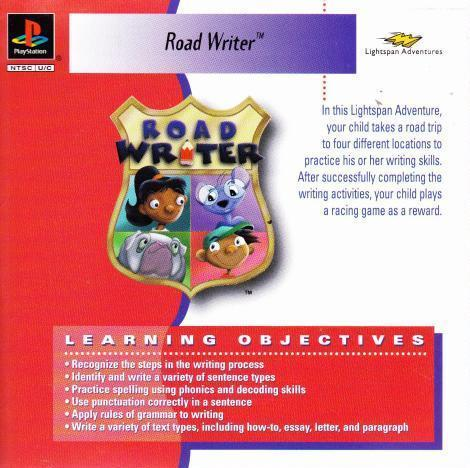
\includegraphics[width=0.5\textwidth]{"./Games/RoadWriter/Images/RoadWriterCDCover.jpg"}
    \caption{Official RoadWriter PlayStation 1 CD Cover}
\end{figure}

Road Writer for the PlayStation 1 is one of the only games within the Lightspan Adventures series that exists on its own as its own game, as opposed to as part of a series.
The game is designed to help children to practice and improve their writing skills.
After successfully completing the writing activities, the player is able to play a racing game as a reward.

The game consists of two difficultly settings: Export and Pro.
Depending on the difficulty the player selects, they will have a variety of different locations to explore within the game.

The Expert difficulty setting has the following locations:

\begin{itemize}
    \item Mount Hans
    \item LaMancha Canyon
    \item Dodgson Creek
    \item New Bronzeville
\end{itemize}

The Pro difficulty setting has the following locations:

\begin{itemize}
    \item Canterbury Canyon
    \item Greene Woods
    \item Hamlet Springs
    \item Hughes City
\end{itemize}

For each location, no matter the difficult, the player is able to select from a variety of writing minigames:

\begin{itemize}
    \item Writing Assignment
    \item Prewriting (contains two difficulties: level 1 and level 2)
    \item Revising (contains two difficulties: level 1 and level 2)
    \item Proofreading (locked until the player has completed the other three minigames)
\end{itemize}
